\chapter{Исследовательский раздел}
\section{Технические характеристики системы}
Исследование поведения системных функций проводилось
на ноутбуке с процессором Intel(R) Core(TM) i5-7200U CPU 2.50 GHz
в виртуальной машине VmWare c 8 гб оперативной памяти под управлением 
операционной системы Linux (дистрибутив Ubuntu 18.04 x86-64, ядро версии 5.0).

\section{Результаты мониторинга процессов}
    % Для исследования поведения перехватываемых системных вызовов в операционной системе Linux
    % был разработан набор приложений, работающие с файлами.
    % \begin{enumerate}
    %     \item Простейшая программа, которая запускается и сразу завершается.
    %     \item Программа, которая открывает первый файл, потом второй и закрывает первый, затем второй.
    %     \item Программа, которая считывает из файла 10 байт.
    %     \item Программа, которая записывает в файл 10 байт.
    %     \item Многопоточная программа, которая записывает в файл 26 байт с потерей данных.
    % \end{enumerate}
    % \subsection*{1) Программа действий не выполняет:}
    1) Программа никаких действий не выполняет (листинг \ref{lst:example:1})
        \begin{lstlisting}[language=C, label=lst:example:1, caption=Программа не выполняющая никаких действий]
int main()
{
    return 0;
}
        \end{lstlisting}

        Система запускает процесс, который ничего не выполняет.
        На рисунке \ref{examples:1out} представлен результат мониторинга системных вызовов
        выполняемых в ходе работы программы.
        
        \begin{figure}[h!]
            \centering
            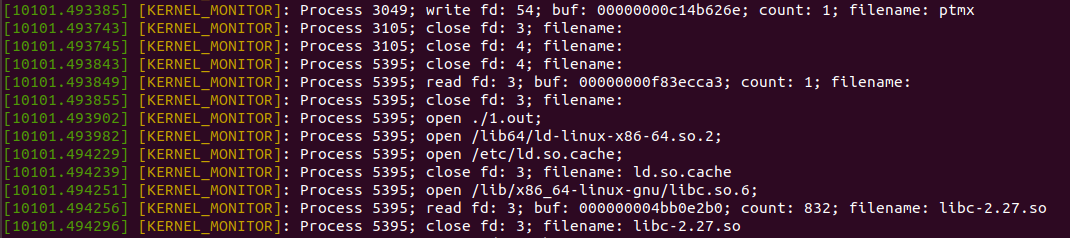
\includegraphics[width = 0.7 \textwidth]{1out.png}
            \caption{Результат мониторинга программы не выполняющей никаких действий.}
            \label{examples:1out}
        \end{figure}

        Из рисунка \ref{examples:1out} видно, что процессы с идентификаторами 3105 (терминал из которого производился запуск программы)
        и 5395 (новый процесс созданный под выполнение программы)
        производят некоторые действия перед открытием исполняемого файла 1.out,
        одно из которых вызовов системного вызова fork для создания процесса программы.
        К сожалению, у некоторых файлов не указывается имя,
        поэтому сложно сказать, какие именно действия производятся 
        %(ниже будет показано, что для других файлов их имена определяются корректно)
        После открытия исполняемого файла происходит загрузка библиотек
        необходимых для работы программы и выполнение кода программы.

        Можно заметить, что не была вызвана функция-обёртка системного вызова
        sys\_open, а только do\_filp\_open, что может быть связано с ассемблерной оптимизацией данного 
        обработчика системного вызова, описанной в аналитическом разделе.

    2) Запускается та же программа (листинг \ref{lst:example:1}),
        но в загружаемый модуль ядра для дополнительного 
        логирования, было добавлено 
        логирование системного вызова get\_unused\_fd\_flags, используя ftrace.

        Из рисунка \ref{examples:1out:alt} видно, что
        файл с исходным кодом 
        открывается с помощью функции do\_filp\_open, а не sys\_open,
        что объясняет отсутствие в лог файле записи о его чтении и закрытии.

        \begin{figure}[h!]
            \centering
            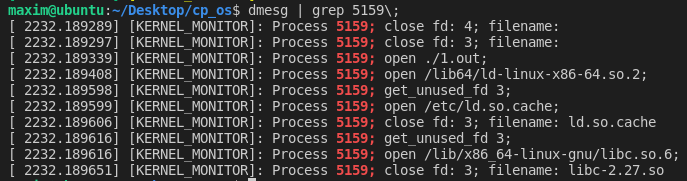
\includegraphics[width = 0.7 \textwidth]{1out-get-fd.png}
            \caption{Результат мониторинга программы не выполняющей никаких действий c дополнительной информацией об открываемом файловом дескрипторе.}
            \label{examples:1out:alt}
        \end{figure}

    3) Программа открывающая и закрывающая файлы (листинг \ref{lst:example:2}).
        \begin{lstlisting}[language=C, label=lst:example:2, caption=Программа открывающая и закрывающая файлы]
#include <fcntl.h>

int main()
{
    int fd1 = open("alphabet.txt", O_RDONLY);
    int fd2 = open("test.txt", O_RDONLY);

    close(fd1);
    close(fd2);
    return 0;
}
        \end{lstlisting}
       
        Система запускает процесс, который открывает существующие файлы alphabet.txt и test.txt,
        после чего закрывает файлы в порядке их открытия.
        
        На рисунке \ref{examples:2out} представлен результат мониторинга системных вызовов,
        выполняемых в ходе работы данной программы.

        Первые 12 строк инициализации процесса были рассмотрены выше.
        Из последних четырёх можно сделать вывод, что
        open возвращает наименьший свободный файловый дескриптор и
        первые три файловых дескрипторов изначально заняты под stdin, stdout, stderr,
        а также корректность определения имени файла по его файловому дескриптору.

        \begin{figure}[h!]
            \centering
            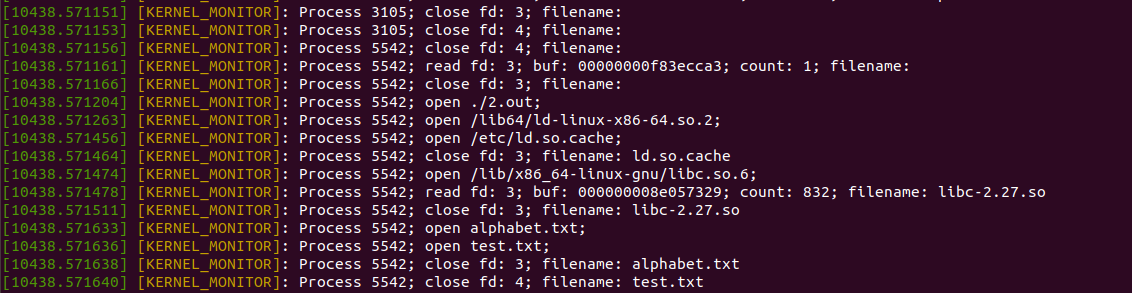
\includegraphics[width = 0.7 \textwidth]{2out.png}
            \caption{Результат мониторинга программы открывающей и закрывающей файлы.}
            \label{examples:2out}
        \end{figure}

    4) Программа с небуферизованным вводом данных (листинг \ref{lst:example:3:alt}).
        \begin{lstlisting}[language=C, label=lst:example:3:alt, caption=Программа с небуфферизованным вводом данных из файла]
#include <fcntl.h>
int main()
{
    int fd = open("alphabet.txt", O_RDONLY);
    char buf[128];

    int len = read(fd, buf, 128);
    buf[len] = 0;
    write(1, buf, len);

    close(fd);
    return 0;
}
        \end{lstlisting}
        
        Система запускает процесс, который открывает существующий файл alphabet.txt
        читает информацию из него, используя системный вызов read, после чего файл закрывается.

        На рисунке \ref{examples:3out:alt} представлен результат мониторинга системных вызовов
        выполняемых в ходе работы данной программы.
        Из рисунка \ref{examples:3out:alt} видно, что небуферизованный ввод использует ровно один вызов функция sys\_read,
        который пытается прочитать из файла 128 байт из открытого файла.

        \begin{figure}[h!]
            \centering
            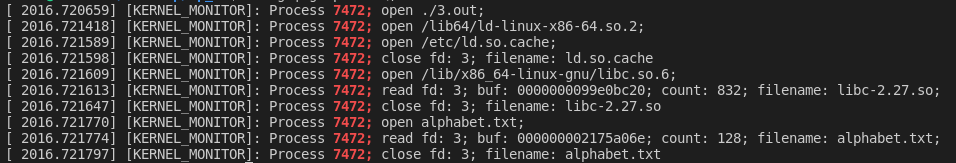
\includegraphics[width = 0.7 \textwidth]{3out-alt.png}
            \caption{Результат мониторинга программы с небуферизованным вводом данных.}
            \label{examples:3out:alt}
        \end{figure}


    5) Программа с буферизованным вводом данных (листинг \ref{lst:example:3}).
        \begin{lstlisting}[language=C, label=lst:example:3, caption=Программа с буфферизованным вводом данных из файла]
#include <stdio.h>

int main()
{
    FILE *f = fopen("alphabet.txt", "r");
    char buf[128];

    fscanf(f, "%s", buf);
    printf("%s", buf);

    fclose(f);
    return 0;
}
        \end{lstlisting}

        Система запускает процесс, который открывает существующий файл alphabet.txt и
        читает информацию из него, используя для этого функцию fscanf
        библиотеки буферизованного ввода/вывода stdio, 
        после чего файл закрывается.

        На рисунке \ref{examples:3out} 
        представлены результаты мониторинга системных вызовов
        выполняемых в ходе работы данной программы.
        
        Из рисунка \ref{examples:3out} видно, что программа с буферизованным вводом дважды
        вызывает системный вызов sys\_read для заполнения буфера размером 4096 байт.

        \begin{figure}[h!]
            \centering
            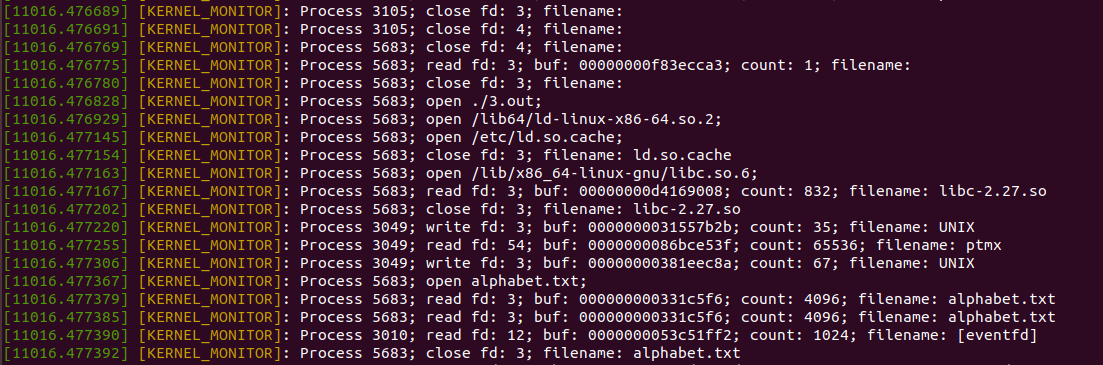
\includegraphics[width = 0.7 \textwidth]{3out.png}
            \caption{Результат мониторинга программы с буферизованным вводом данных.}
            \label{examples:3out}
        \end{figure}

    6) Программа, которая записывает информацию в файл, используя библиотеку буферизованного ввода/вывода (листинг \ref{lst:example:4}).
        \begin{lstlisting}[language=C, label=lst:example:4, caption=Программа с буферизованным выводом данных в файл]
#include <stdio.h>

int main()
{
    FILE *f = fopen("test.txt", "w");
    char buf[128] = "1234567890";
    fprintf(f, "%s", buf);
    fprintf(f, "%s", buf);
    fclose(f);
    return 0;
}
        \end{lstlisting}

        Система запускает процесс, который открывает файл test.txt и
        два раза записывает в него по 10 байт, используя для этого функцию fprintf
        библиотеки буферизованного ввода/вывода stdio, 
        после чего файл закрывается.

        На рисунке \ref{examples:4out} представлен результат мониторинга системных вызовов
        выполняемых в ходе работы данной программы, из которого видно, 
        что системный вызов sys\_write был вызван единожды на запись 20 байт,
        т.к. использовался буфер на 4096 байт, который записывается в файл, 
        либо если буфер полностью заполнен, либо файл закрывается.

        \begin{figure}[h!]
            \centering
            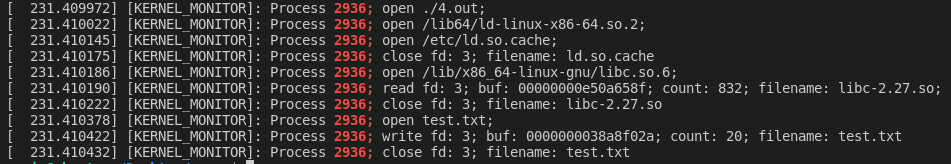
\includegraphics[width = 0.7 \textwidth]{4out-alt.png}
            \caption{Результат мониторинга программы с буферизованным вывод данных.}
            \label{examples:4out}
        \end{figure}

    7) Многопоточная программа, которая записывает в файл с потерей данных (листинг \ref{lst:example:5}).        
        \begin{lstlisting}[language=C, label=lst:example:5, caption=Многопоточная программа записывающая данные в один файл]
#include <stdio.h>
#include <sys/stat.h>
#include <pthread.h>

#define THREADS 4
void *write_file(void *arg)
{
    int num = (int)arg;
    struct stat statbuf;
    FILE *f = fopen("write_thread.txt", "w");

    for (char c = 'a' + num; c <= 'z'; c += THREADS)
        fprintf(f, "%c", c);

    fclose(f);
    return 0;   
}

int main()
{
    pthread_t threads[THREADS];

    for (int i = 0; i < THREADS; i++) 
    {
        int code = pthread_create(threads + i, NULL, write_file, i);
        if (code != 0)
        {
            printf("can't create thread, code = %d\n", code);
            return code;
        }
    }
    
    for (int i = 0; i < THREADS; i++) 
        pthread_join(threads[i], NULL);
    return 0;
}
        \end{lstlisting}

        Проанализируем поведение перехватываемых функций, в случае многопоточной обработки файла.
        Для этого была реализована пятая программа ,
        которая в несколько потоков записывает данные в один файл с потерей данных.

        Система запускает процесс, который в четыре потока,
        открывает файл write\_thread.txt  и записывает в него информацию с потерей данных.
        
        На рисунке \ref{examples:5out} представлен отфильтрованный результат мониторинга системных вызовов
        выполняемых в ходе работы данной программы.
        Из него можно сделать вывод, что потоки в линуксе на самом деле реализованы в виде процессов.

    \begin{figure}[h!]
        \centering
        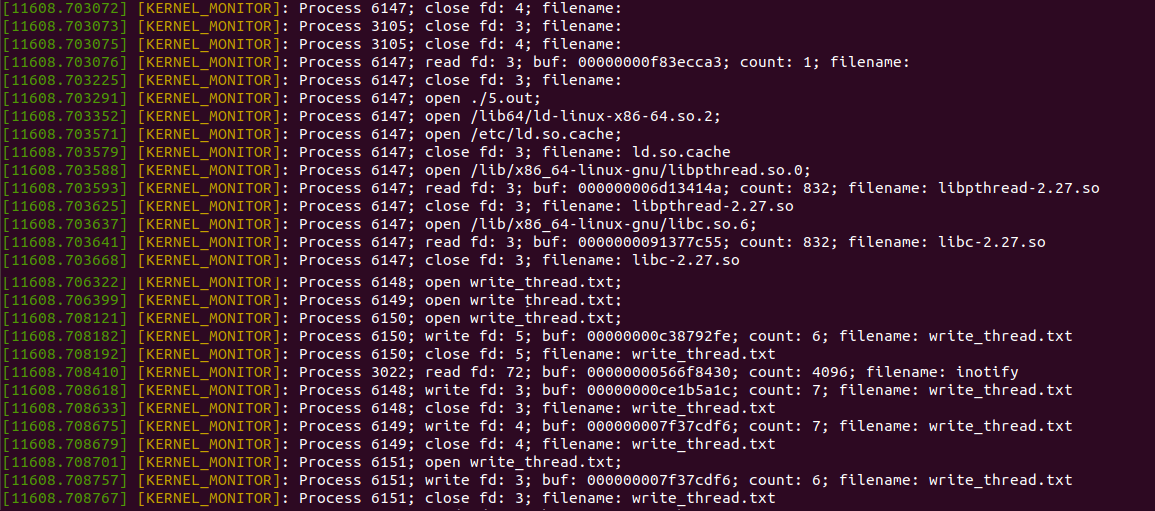
\includegraphics[width = 0.7 \textwidth]{5out-alt.png}
        \caption{Результат мониторинга многопоточной программы записывающая данные в файл с потерей данных.}
        \label{examples:5out}
    \end{figure}

\pagebreak